\documentclass[11pt,a4paper]{article}
\usepackage[margin=17mm,headheight=14pt]{geometry}
\usepackage[T1]{fontenc}
\usepackage{needspace}
\usepackage{lmodern,microtype,booktabs,tabularx,array,xcolor,hyperref,fancyhdr}
\usepackage{tikz}
\usetikzlibrary{positioning,arrows.meta}
\hypersetup{colorlinks=true,urlcolor=blue!50!black,linkcolor=black}
\setlength{\parindent}{0pt}
\setlength{\parskip}{4pt}
\setlength{\emergencystretch}{3em}
\newcommand{\rp}[1]{\path{#1}}
\newcommand{\subhead}[1]{\Needspace{5\baselineskip}\vspace{0.5em}\noindent{\bfseries #1}\par\vspace{-0.1em}}
\pagestyle{fancy}\fancyhf{}\lhead{\small ARIADNE / COOL EVIDENCE}\rhead{\small OpenCV AI Competition 2026}\cfoot{\thepage}
\begin{document}
\begin{center}
{\Large\bfseries Cloud-Optimized Vision on AWS Graviton4}\\[3pt]
{\small Ariadne | Best Use of COOL award evidence | Technical companion to the main report}
\end{center}
\vspace{-0.6em}

\subhead{The workload that repeats}
Ariadne's stereo agents acquire a new image every $50$\,ms of simulated time. Each frame passes through camera rectification, photometric preparation, pyramidal Lucas--Kanade (LK) tracking and stereo processing; selected keyframes additionally invoke OpenCV DNN recognition and geometric verification. The cost of these recurring image operations multiplies with the number of agents. Ariadne therefore isolates the OpenCV hot path for native Arm execution, while retaining stereo-inertial estimation, graph optimization, communications and route planning above stable C++ interfaces.

The COOL comparison is anchored to operations that remain useful in the adopted tracker: \texttt{cv::remap}, pyramid construction, \texttt{cv::calcOpticalFlowPyrLK}, pixel conversion and resizing. Flat-field multiplication, variance-stabilizing transforms and restoration form separately identified radiometric configurations; feature serialization and descriptor indexing are timed at the pipeline boundary without attributing their entire cost to COOL. This workload choice survives the algorithm ablations: XFeat was accurately ported to OpenCV DNN but regressed EuRoC VO on six of seven tested flights, and optional image normalization offered no trajectory gain. ORB/LK continues to supply the high-frequency geometric evidence.

\begin{center}
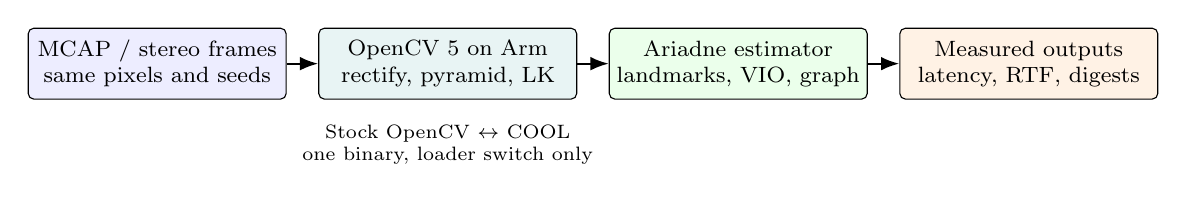
\begin{tikzpicture}[>=Latex,node distance=4mm and 4mm, every node/.style={font=\footnotesize},
 b/.style={draw,rounded corners=2pt,align=center,minimum height=9mm,text width=31mm,inner sep=2.5pt}]
 \node[b,fill=blue!7] (rec) {MCAP / stereo frames\\same pixels and seeds};
 \node[b,fill=teal!9,right=of rec] (cv) {OpenCV 5 on Arm\\rectify, pyramid, LK};
 \node[b,fill=green!8,right=of cv] (est) {Ariadne estimator\\landmarks, VIO, graph};
 \node[b,fill=orange!10,right=of est] (res) {Measured outputs\\latency, RTF, digests};
 \draw[->,thick] (rec)--(cv);\draw[->,thick] (cv)--(est);\draw[->,thick] (est)--(res);
 \node[below=2mm of cv,align=center,font=\scriptsize] {Stock OpenCV $\leftrightarrow$ COOL\\one binary, loader switch only};
\end{tikzpicture}
\end{center}

\subhead{COOL version and AWS configuration}
\begin{center}\footnotesize
\begin{tabularx}{\linewidth}{@{}p{38mm}X@{}}
\toprule
COOL product & AWS Marketplace \emph{Cloud Optimized OpenCV for Graviton4} (\url{https://aws.amazon.com/marketplace/pp/prodview-fdvbfiewzuehs}): COOL 3.1, an OpenCV 5.x build for Neoverse-V2 with KleidiCV and Arm Performance Libraries, Ubuntu 24.04; C++ SDK under \rp{/opt/cool/cpp_sdk}.\\
AMI (as published) & \texttt{Graviton5-COOL-v3-prod-k6u24vxijyzvg}; eu-north-1 \texttt{ami-0a302ff85af8d8764}, published in 18 regions (\rp{build/cool-regions.tsv}; DECISIONS D28). The AMI name and the listing version label (3.1) are the vendor's.\\
Instance & c8g.4xlarge (Graviton4, Neoverse-V2, 16 vCPU), eu-north-1, spot; \texttt{spinup.sh} profile \texttt{cool} (\rp{infra/scripts/spinup.sh}). m8g.4xlarge is the design's concurrent-agent throughput instance (arch \S26.3).\\
Pinned OpenCV & 5.0.0; opencv \texttt{40738fb16ced}, opencv\_contrib \texttt{755e50675d97} (\rp{infra/docker/opencv-base.Dockerfile}); x86 build hash \texttt{fnv1a64:cf8ea084bb984703}. C++17, Eigen 3.4.1, gcc 13.3, \texttt{-O3 -ffp-contract=off}.\\
Stock Arm HAL & The stock arm64 build already enables carotene + KleidiCV 26.03; dispatch \texttt{NEON FP16 *NEON\_DOTPROD *NEON\_FP16 *NEON\_BF16} (\rp{evaluation/runs/arm64/20261023T193621Z-cpuarm-7f8c96/opencv_hal_simd.txt}). A stock-versus-COOL pair is therefore KleidiCV-stock versus COOL.\\
\bottomrule
\end{tabularx}\end{center}

\subhead{Execution identity: one binary, loader switch only}
Ariadne's build enforces \texttt{ARIADNE\_REQUIRE\_OPENCV=ON} for the full OpenCV-linked target set (root \rp{CMakeLists.txt}). \texttt{CMAKE\_SKIP\_RPATH=ON} and an installed-binary \texttt{readelf} gate (\rp{infra/docker/core.Dockerfile}) refuse any embedded RPATH/RUNPATH that would silently defeat the library switch. At execution the manifest records the OpenCV version, \texttt{cv::getCPUFeaturesLine()} and an FNV-1a digest of \texttt{cv::getBuildInformation()} taken from the \emph{loaded} \texttt{libopencv\_core}; \texttt{/proc/self/maps} names the shared objects actually mapped. The same binary therefore runs on stock OpenCV or on COOL by changing \texttt{LD\_LIBRARY\_PATH} alone, and the manifest proves which one processed the frames.

\begin{small}\begin{verbatim}
# Build against the COOL SDK on the Graviton4 AMI (or against stock, then switch the loader):
cmake -S . -B build/cool -DARIADNE_REQUIRE_OPENCV=ON \
      -DOpenCV_DIR=/opt/cool/cpp_sdk/lib/cmake/opencv4 -DCMAKE_SKIP_RPATH=ON
cmake --build build/cool -j
LD_LIBRARY_PATH=/opt/cool/cpp_sdk/lib:$LD_LIBRARY_PATH build/cool/<target>   # COOL
LD_LIBRARY_PATH=/opt/stock/lib:$LD_LIBRARY_PATH        build/cool/<target>   # stock
\end{verbatim}\end{small}

\subhead{Evaluation method (\rp{infra/cool/day1.sh}, \rp{infra/cool/probe.cpp})}
One command launches the protocol on a fresh COOL instance and writes every step's evidence as it completes:
\begin{small}\begin{verbatim}
infra/scripts/spinup.sh run --profile cool --type c8g.4xlarge --max-minutes 90 -- 'bash infra/cool/day1.sh'
\end{verbatim}\end{small}
\vspace{-0.4em}
\begin{enumerate}\setlength{\itemsep}{1pt}
\item Inspect \rp{/opt/cool}: layout, sonames, CMake package, COOL's own build information and module list.
\item Build stock OpenCV 5.0.0 + contrib natively on the same instance, at the pinned commits with the exact module list and flags of the project image, into \rp{/opt/stock}.
\item Loader-switch probe: one binary built against stock, run with stock and with \rp{/opt/cool/cpp_sdk/lib} first; \texttt{/proc/self/maps} gates ``same binary, loader switch only''.
\item Per-operation output checksums and timings at 1 thread and at all cores, on a $1280\times720$ frame with the tracker's parameters: \texttt{cvtColor}, \texttt{remap} (linear), \texttt{resize} (area, half size), \texttt{GaussianBlur} $5\times5$, \texttt{pyrDown}, \texttt{buildOpticalFlowPyramid} and \texttt{calcOpticalFlowPyrLK} (window 21, 3 levels), \texttt{Sobel}, Otsu \texttt{threshold}.
\end{enumerate}
The whole-pipeline stage then replays one recorded stereo MCAP through the same binary on both libraries (the replay harness is the one every Ariadne run uses), reporting p50/p95 per-frame latency, frames per second, CPU utilization, the trajectory digest and pose tolerances.
Cost per frame is reported as $C_{\mathrm{frame}}=(C_{\mathrm{instance/h}}+C_{\mathrm{software/h}})/(3600\,\mathrm{FPS})$ with the actual spot and Marketplace prices. Labels stay separate for stock-x86, stock-Arm and COOL-Arm; restoration-only configurations remain auxiliary.

\subhead{Graviton4 results (stock OpenCV 5.0.0, measured)}
\begin{center}\footnotesize
\begin{tabularx}{\linewidth}{@{}p{36mm}p{62mm}X@{}}
\toprule
\textbf{Check} & \textbf{Result} & \textbf{Evidence}\\
\midrule
Native arm64 build + full test suite & OpenCV 5.0.0 + contrib built natively; \textbf{708/708} C++ tests pass on the consolidated tree; image gate PASS; commits match the Dockerfile. 901\,s, about \$0.02. & c8g.4xlarge run \texttt{20261024T100530Z-cpuarm-602802}, \rp{evaluation/runs/arm64/20261024T100530Z-cpuarm-602802/}\\
Cross-architecture determinism & Replay digests identical between x86 and Graviton. & \rp{docs/SMOKE_TEST_RESULTS.md} \S4e (run \texttt{20260929T145114Z-cpu-762cb1})\\
Wire bytes across architectures & A FlatBuffers child-construction order difference made arm64 bytes differ; fixed so both architectures emit identical goldens. & commit \texttt{6a16717}; arm64 run \texttt{05b8cc}\\
Learned kernels, Arm vs x86 & ALIKED $1280\times720$: \textbf{530\,ms on c8g vs 829\,ms on c7i} (16 threads, ratio 0.64); LightGlue / EigenPlaces ratio 0.85--0.88. & \rp{evaluation/runs/perf/pipeline_profile_20261024/} item 10\\
Thread invariance & Estimator output identical at OpenCV thread settings 2, 5 and 16; three-agent replay RTF 0.836 on c7i.4xlarge. & main report, \S Compute profile\\
\bottomrule
\end{tabularx}\end{center}

\subhead{Published COOL figures (vendor, for context)}
AWS reports an image-analysis workflow at 1.6\,fps on COOL against 1.2\,fps with pip-installed OpenCV 4.12 on Graviton4 (about 30\%), and up to 70\% faster core operations (resize, adaptive Gaussian filtering, contour detection) across 78 functions (\url{https://aws.amazon.com/blogs/spatial/accelerating-opencv-on-graviton-the-cool-framework}; \url{https://opencv.org/cool/}). Those baselines are pip OpenCV~4.12; Ariadne's stock baseline is OpenCV~5.0.0 with KleidiCV already enabled, so the protocol above measures COOL against the stronger reference.

\subhead{Evidence entry points}
Build and loader controls: \rp{infra/docker/core.Dockerfile}, \rp{infra/docker/opencv-base.Dockerfile}, \rp{docker-bake.hcl}, \rp{infra/scripts/core.sh}, \rp{infra/cool/day1.sh}, \rp{infra/cool/probe.cpp}, \rp{infra/scripts/spinup.sh}, root \rp{CMakeLists.txt}. Workload definition: \rp{docs/ARIADNE_IMPLEMENTATION_ARCHITECTURE.md} \S\S26.3, 27.1, 38.1 and Iteration~14. Arm runs: \rp{evaluation/runs/arm64/}. x86 integration: \rp{evaluation/runs/premerge_aws/20261024T083919Z-cpux86-73e3fa/} (54/54 checks).

\emph{Judge verification:} subscribe to the COOL AMI, run the one-command protocol above, and compare the two manifests: the loaded-library list and build-information digest identify stock or COOL, the input digest proves identical frames, and the per-operation and whole-pipeline tables give the speedup at matched outputs.
\end{document}
